
\chapter{Arquitetura de Software}
\label{sec-arquitetura}

A arquitetura de software do sistema~\imprimirtitulo{} segue uma arquitetura análoga à padrão sugerida pelo FrameWeb~\cite{souza:masterthesis07,souza-et-al:iism09} baseada no padrão Camada de Serviço~\cite{fowler:book02}. A Figura~\ref{figura-arquitetura-padrao} ilustra tal arquitetura sugerida e indica onde atuariam os \textit{frameworks} para desenvolvimento Web Java com \textit{JSF}, \textit{JPA}, \textit{CDI}, \textit{PrimeFaces} e \textit{Facelets}.

\begin{figure}[h]
	\centering
	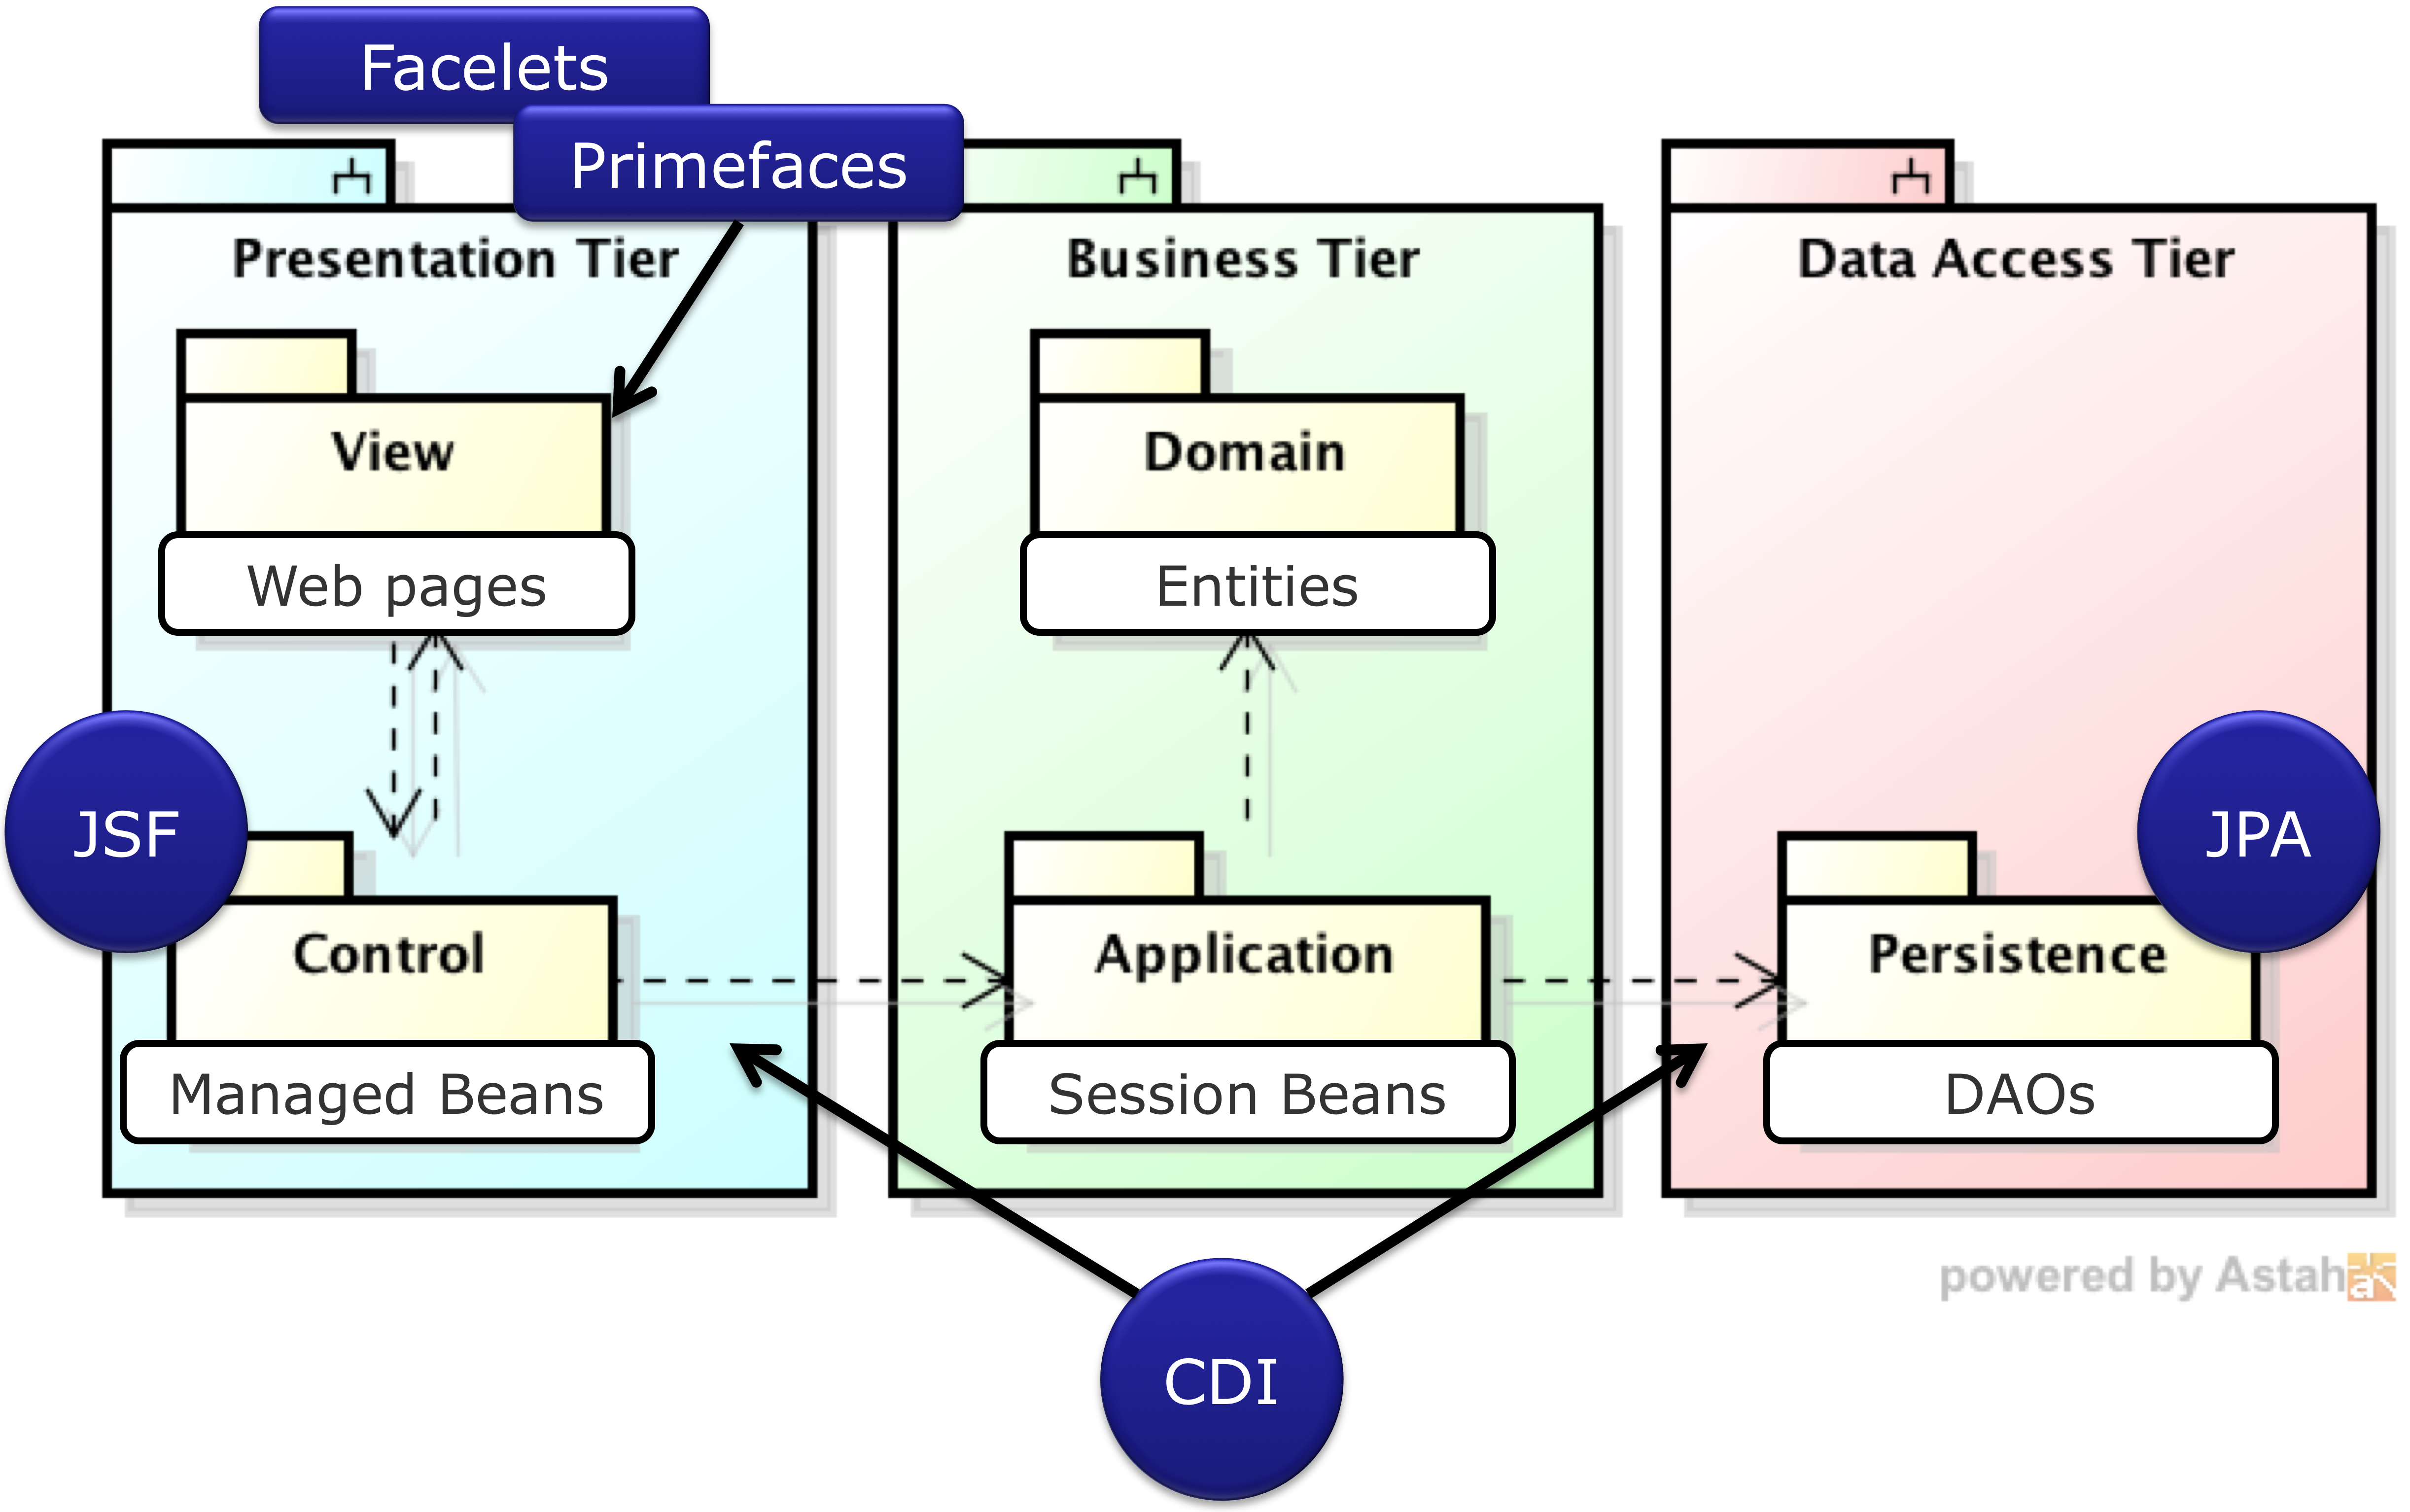
\includegraphics[width=0.7\textwidth]{figuras/figura-arquitetura-padrao.png}
	\caption{Arquitetura padrão proposta pelo FrameWeb.}
	\label{figura-arquitetura-padrao}
\end{figure}

Entretanto, como tal arquitetura não se mantém no padrão Django, que é composta de \textit{models}, \textit{views} e \textit{templates} com responsabilidades diferentes da dos elementos de mesmo nome na arquitetura Java EE. Portanto é necessario fazer aproximações para ambos os modelos dizerem a mesma coisa com palavras diferentes. Se adicionarmos uma camada de serviços entre os \textit{models} e \textit{views}, podemos obter uma arquitetura como a da figura \ref{figura-arquitetura-adaptada}, que é bastante similar à \ref{figura-arquitetura-padrao}. Como Django usa Active Record e não Data Access Objects, a camada de acesso ao dado foi ignorada.

\begin{figure}[h]
	\centering
	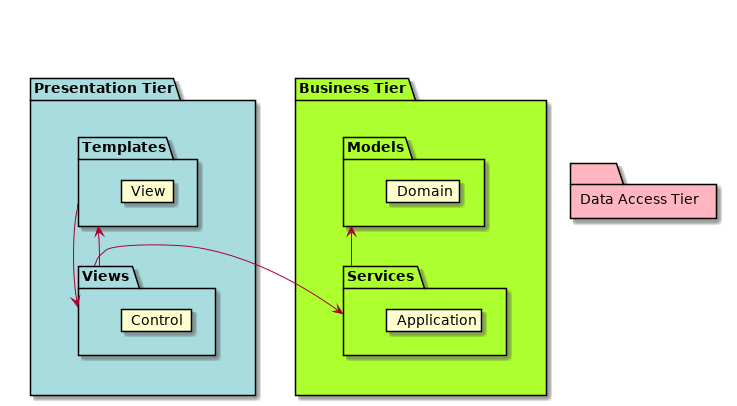
\includegraphics[width=0.7\textwidth]{figuras/arquitetura.png}
	\caption{Arquitetura que busca aproximar o modelo do Django à do FrameWeb.}
	\label{figura-arquitetura-adaptada}
\end{figure}

Nas próximas seções, serão apresentados diagramas FrameWeb relativos a cada uma das camadas da arquitetura do sistema.


\section{Camada de Apresentação}
\label{sec-arquitetura-apresentacao}

% \vitor{Apresentar os modelos de navegação do FrameWeb.}

\begin{figure}[H]
	\centering
	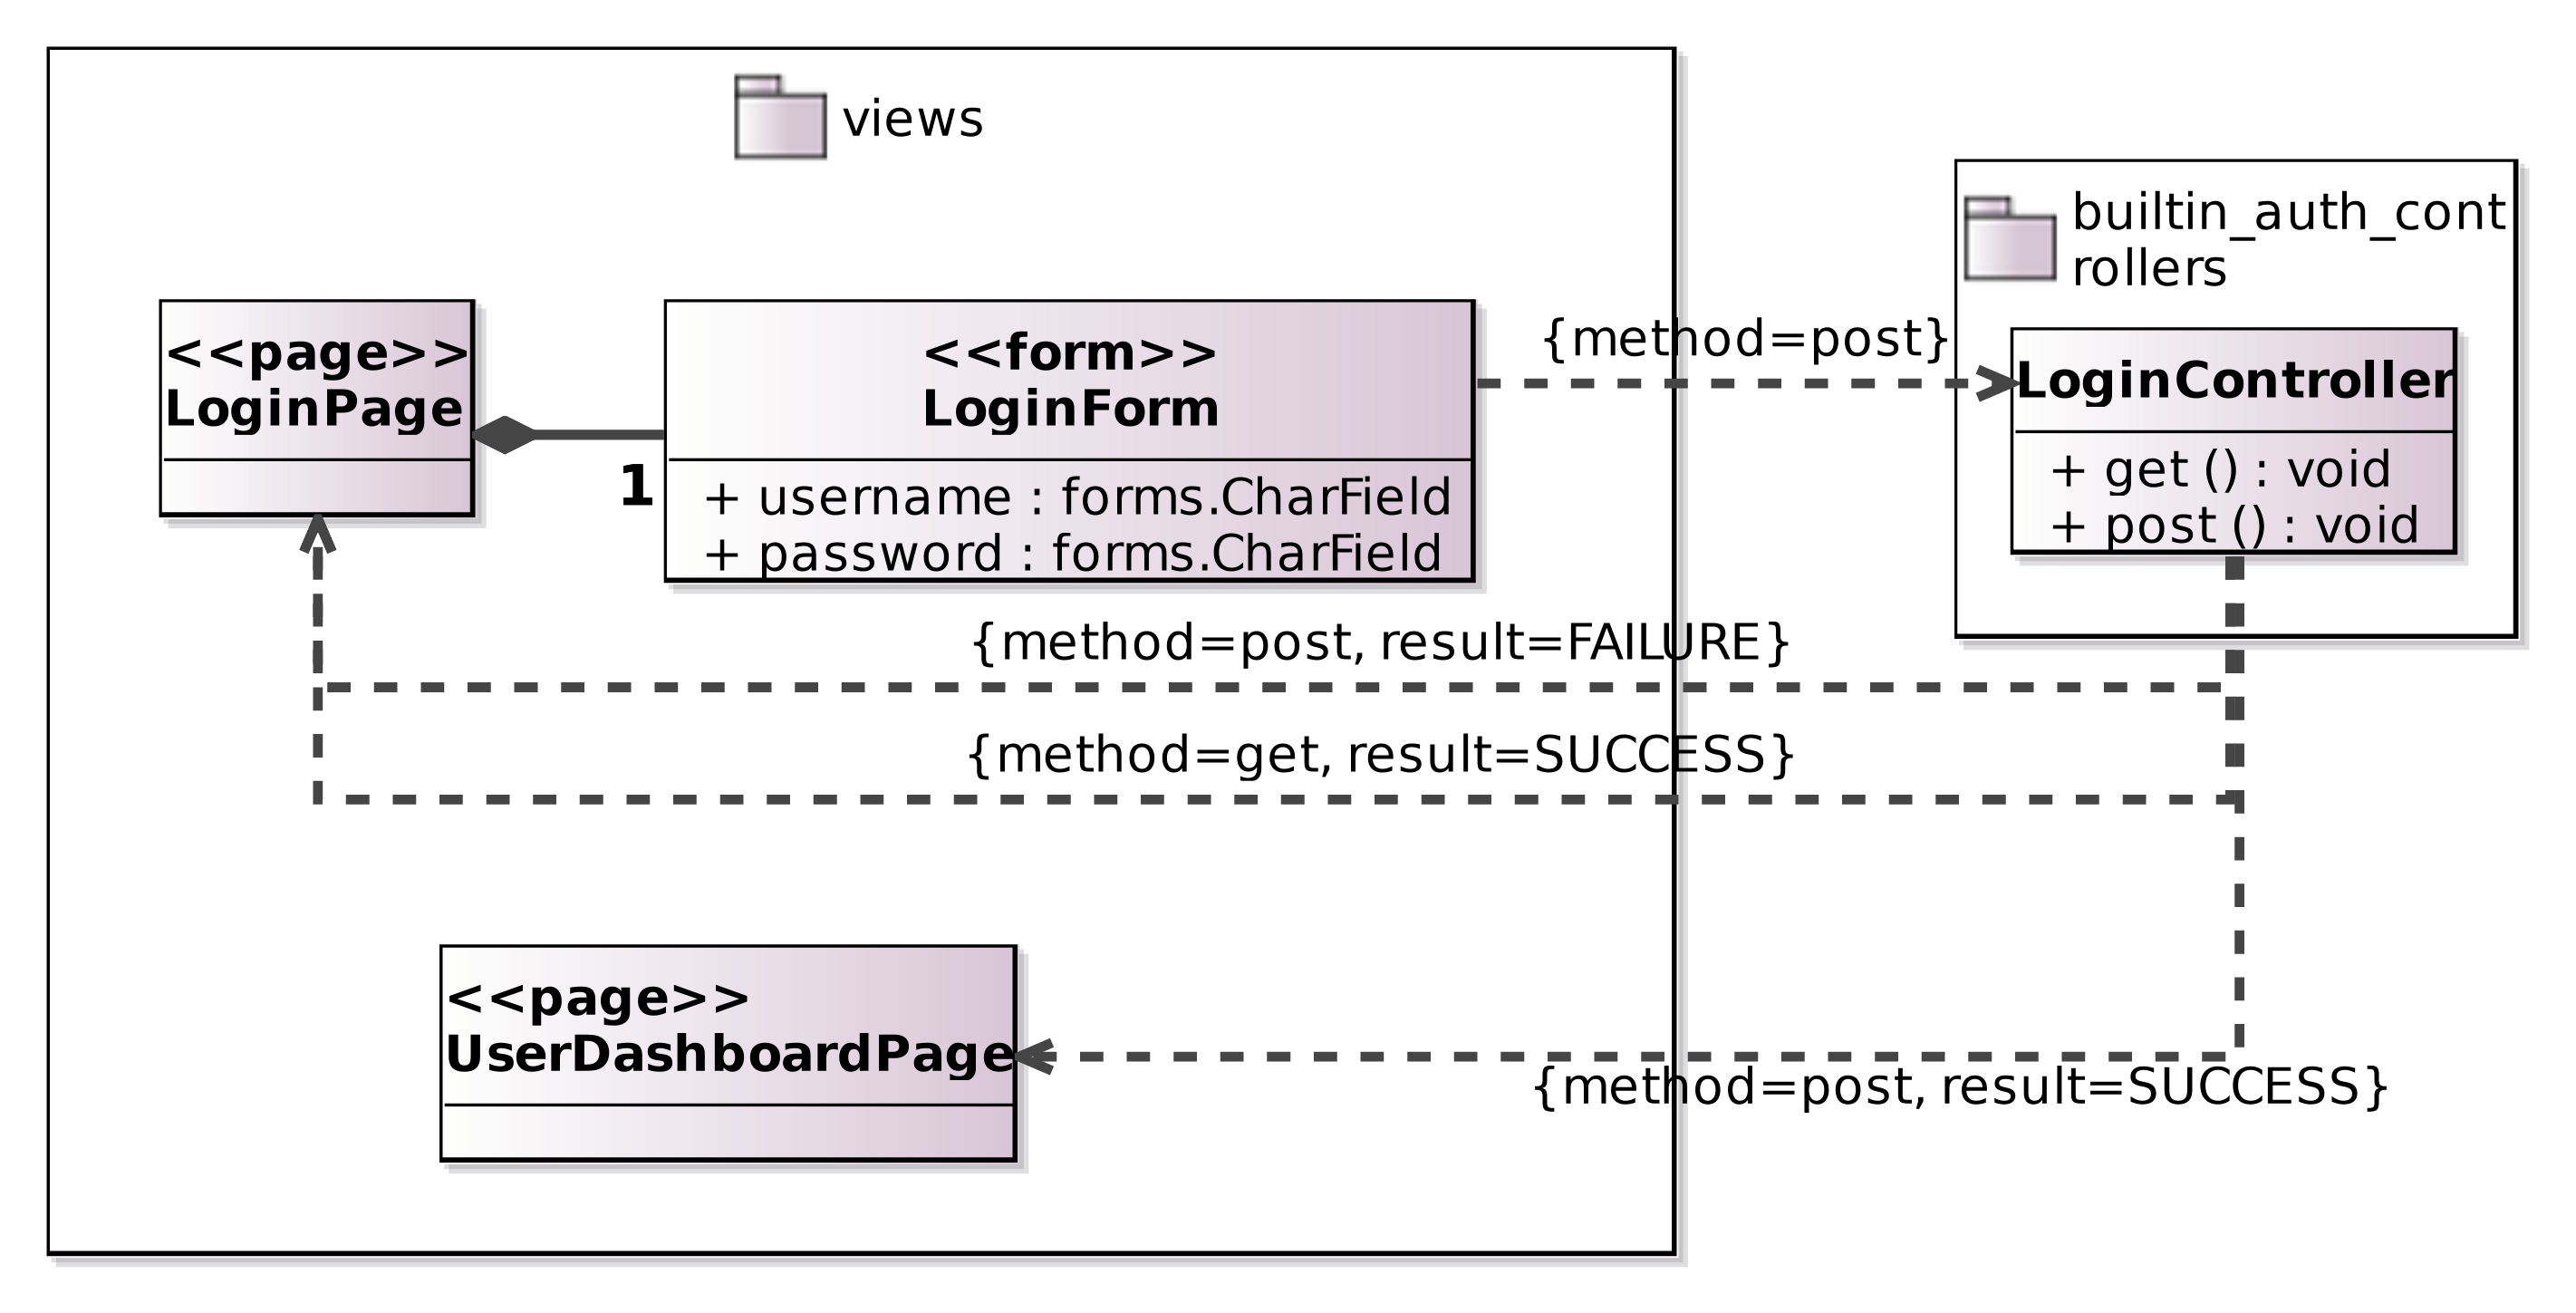
\includegraphics[scale=0.15]{figuras/FrameWebNavigationModel1.jpg}
	\caption{Modelo de Navegação do \imprimirtitulo{} -- Login}
	\label{fig:nav1}
\end{figure}

\begin{figure}[H]
	\centering
	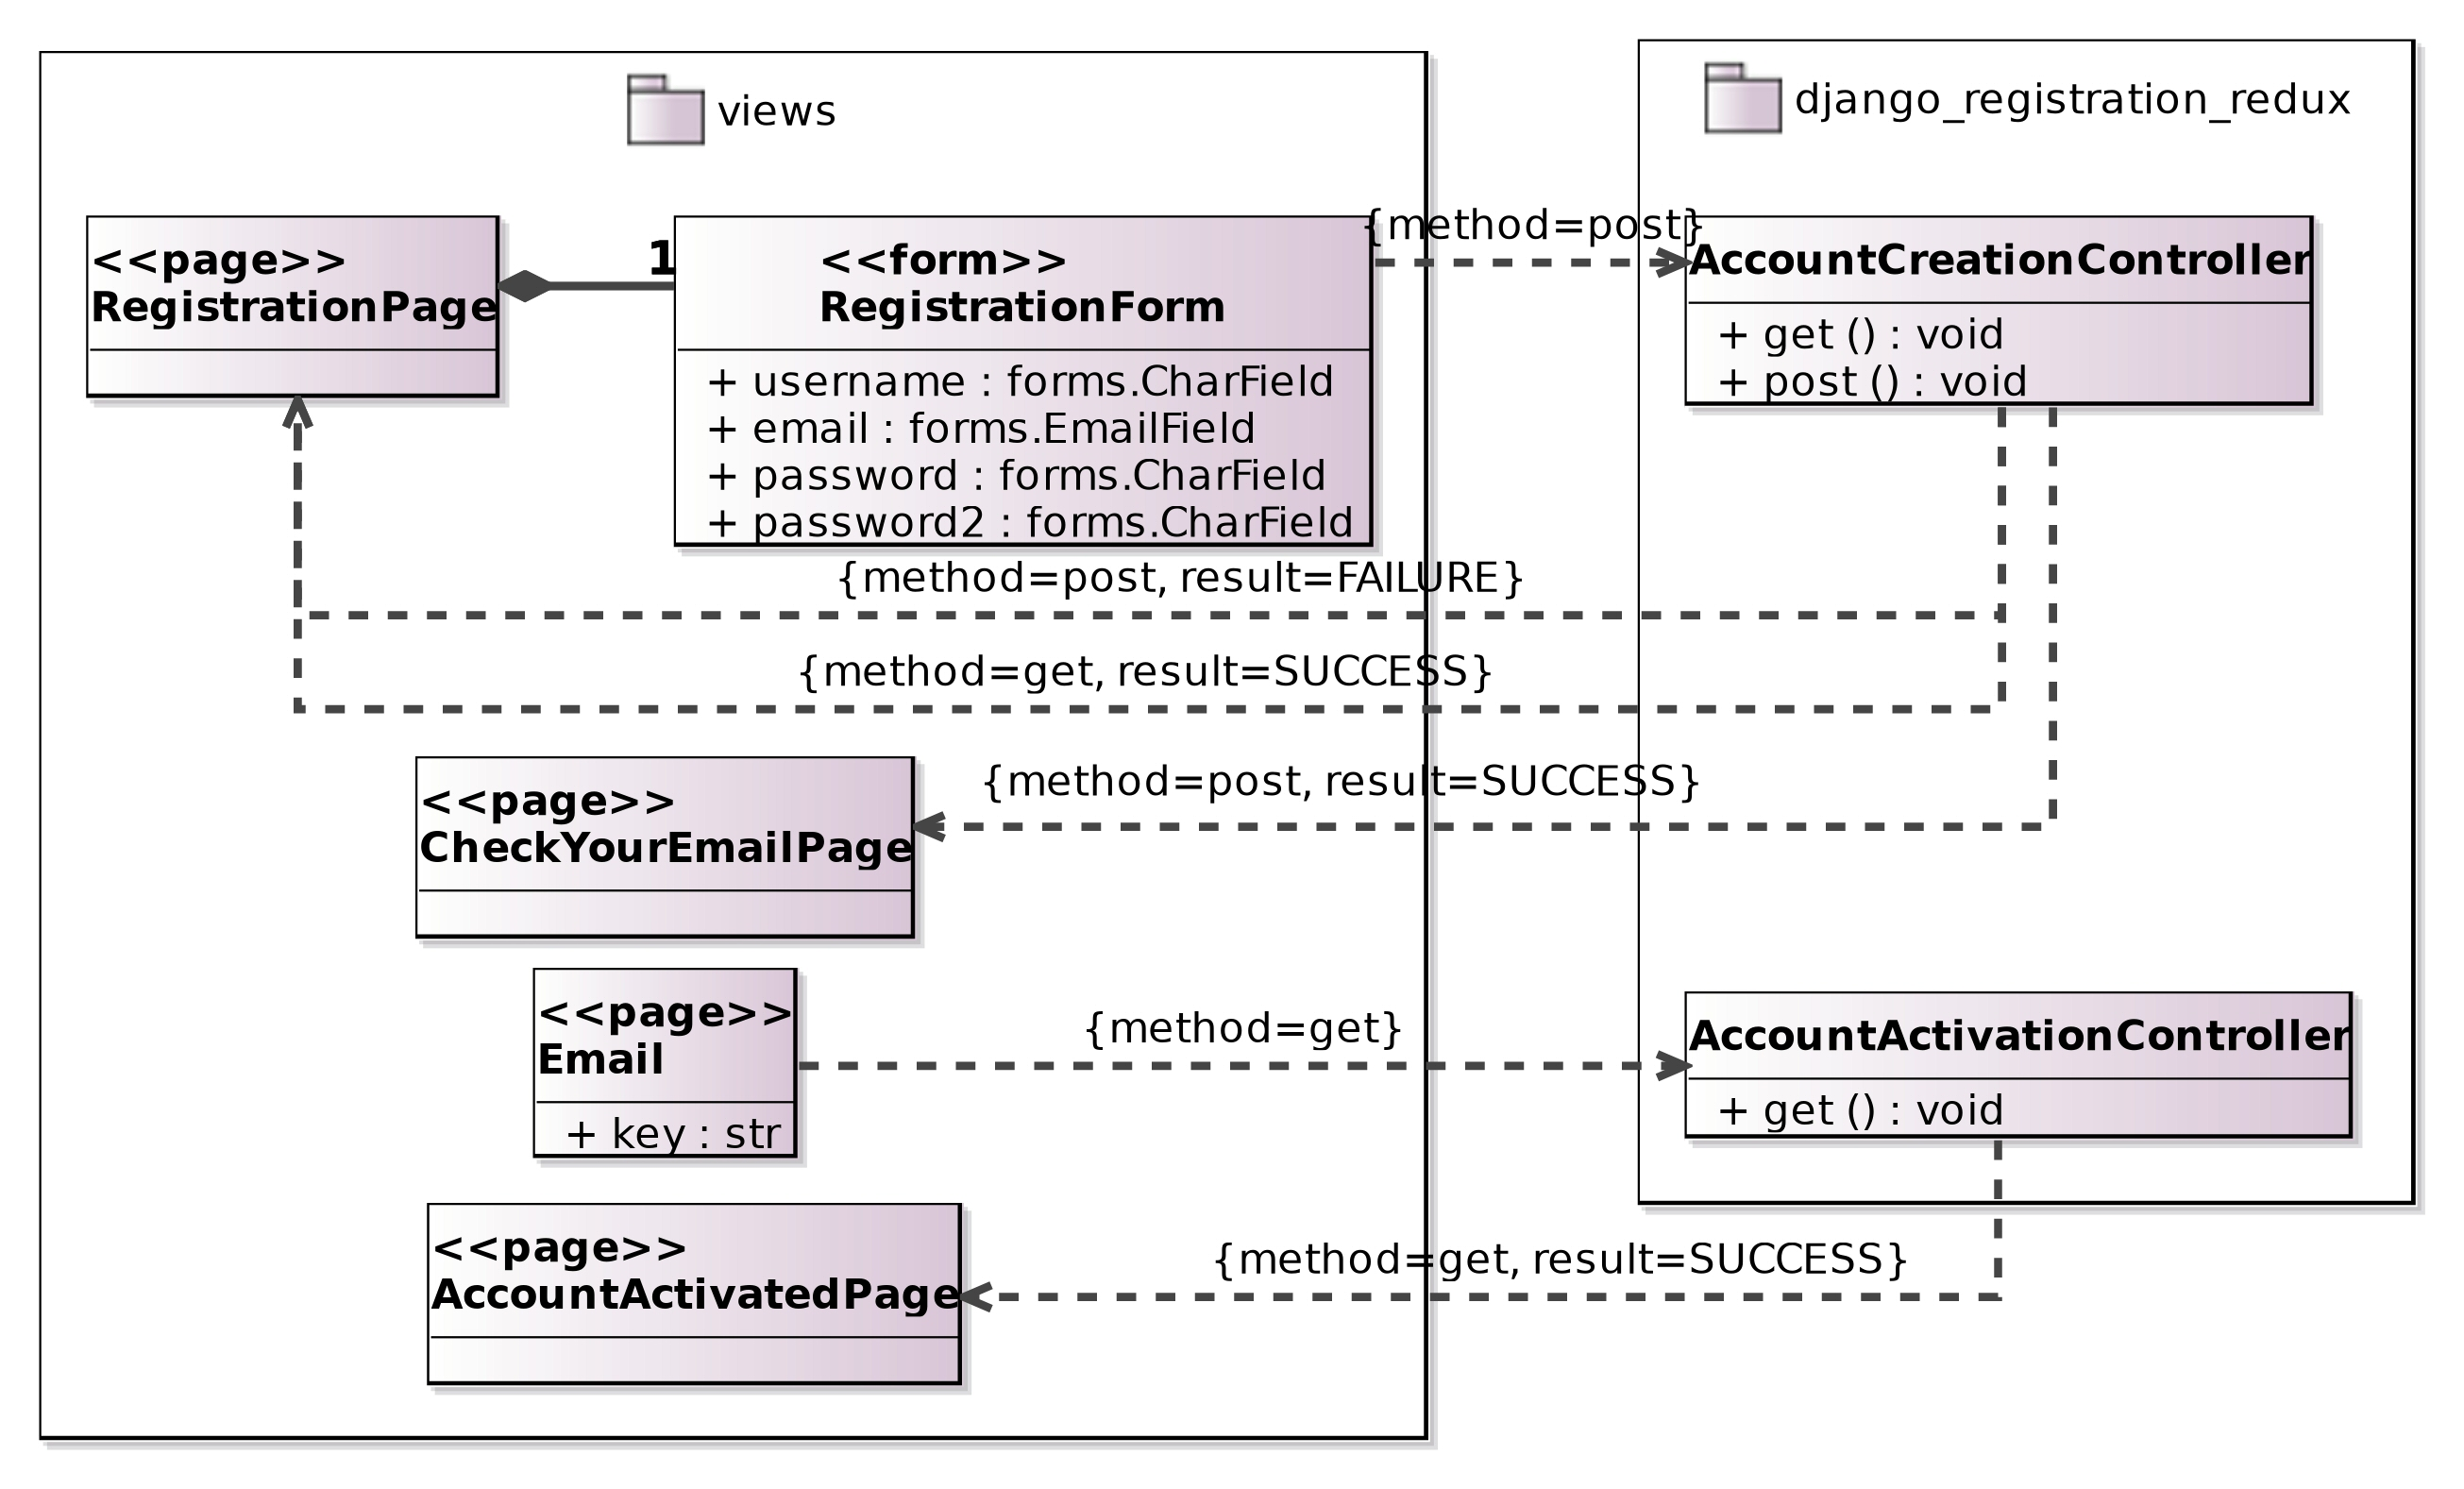
\includegraphics[scale=0.15]{figuras/FrameWebNavigationModel2.jpg}
	\caption{Modelo de Navegação do \imprimirtitulo{} -- Criar conta}
	\label{fig:nav2}
\end{figure}

\begin{figure}[H]
	\centering
	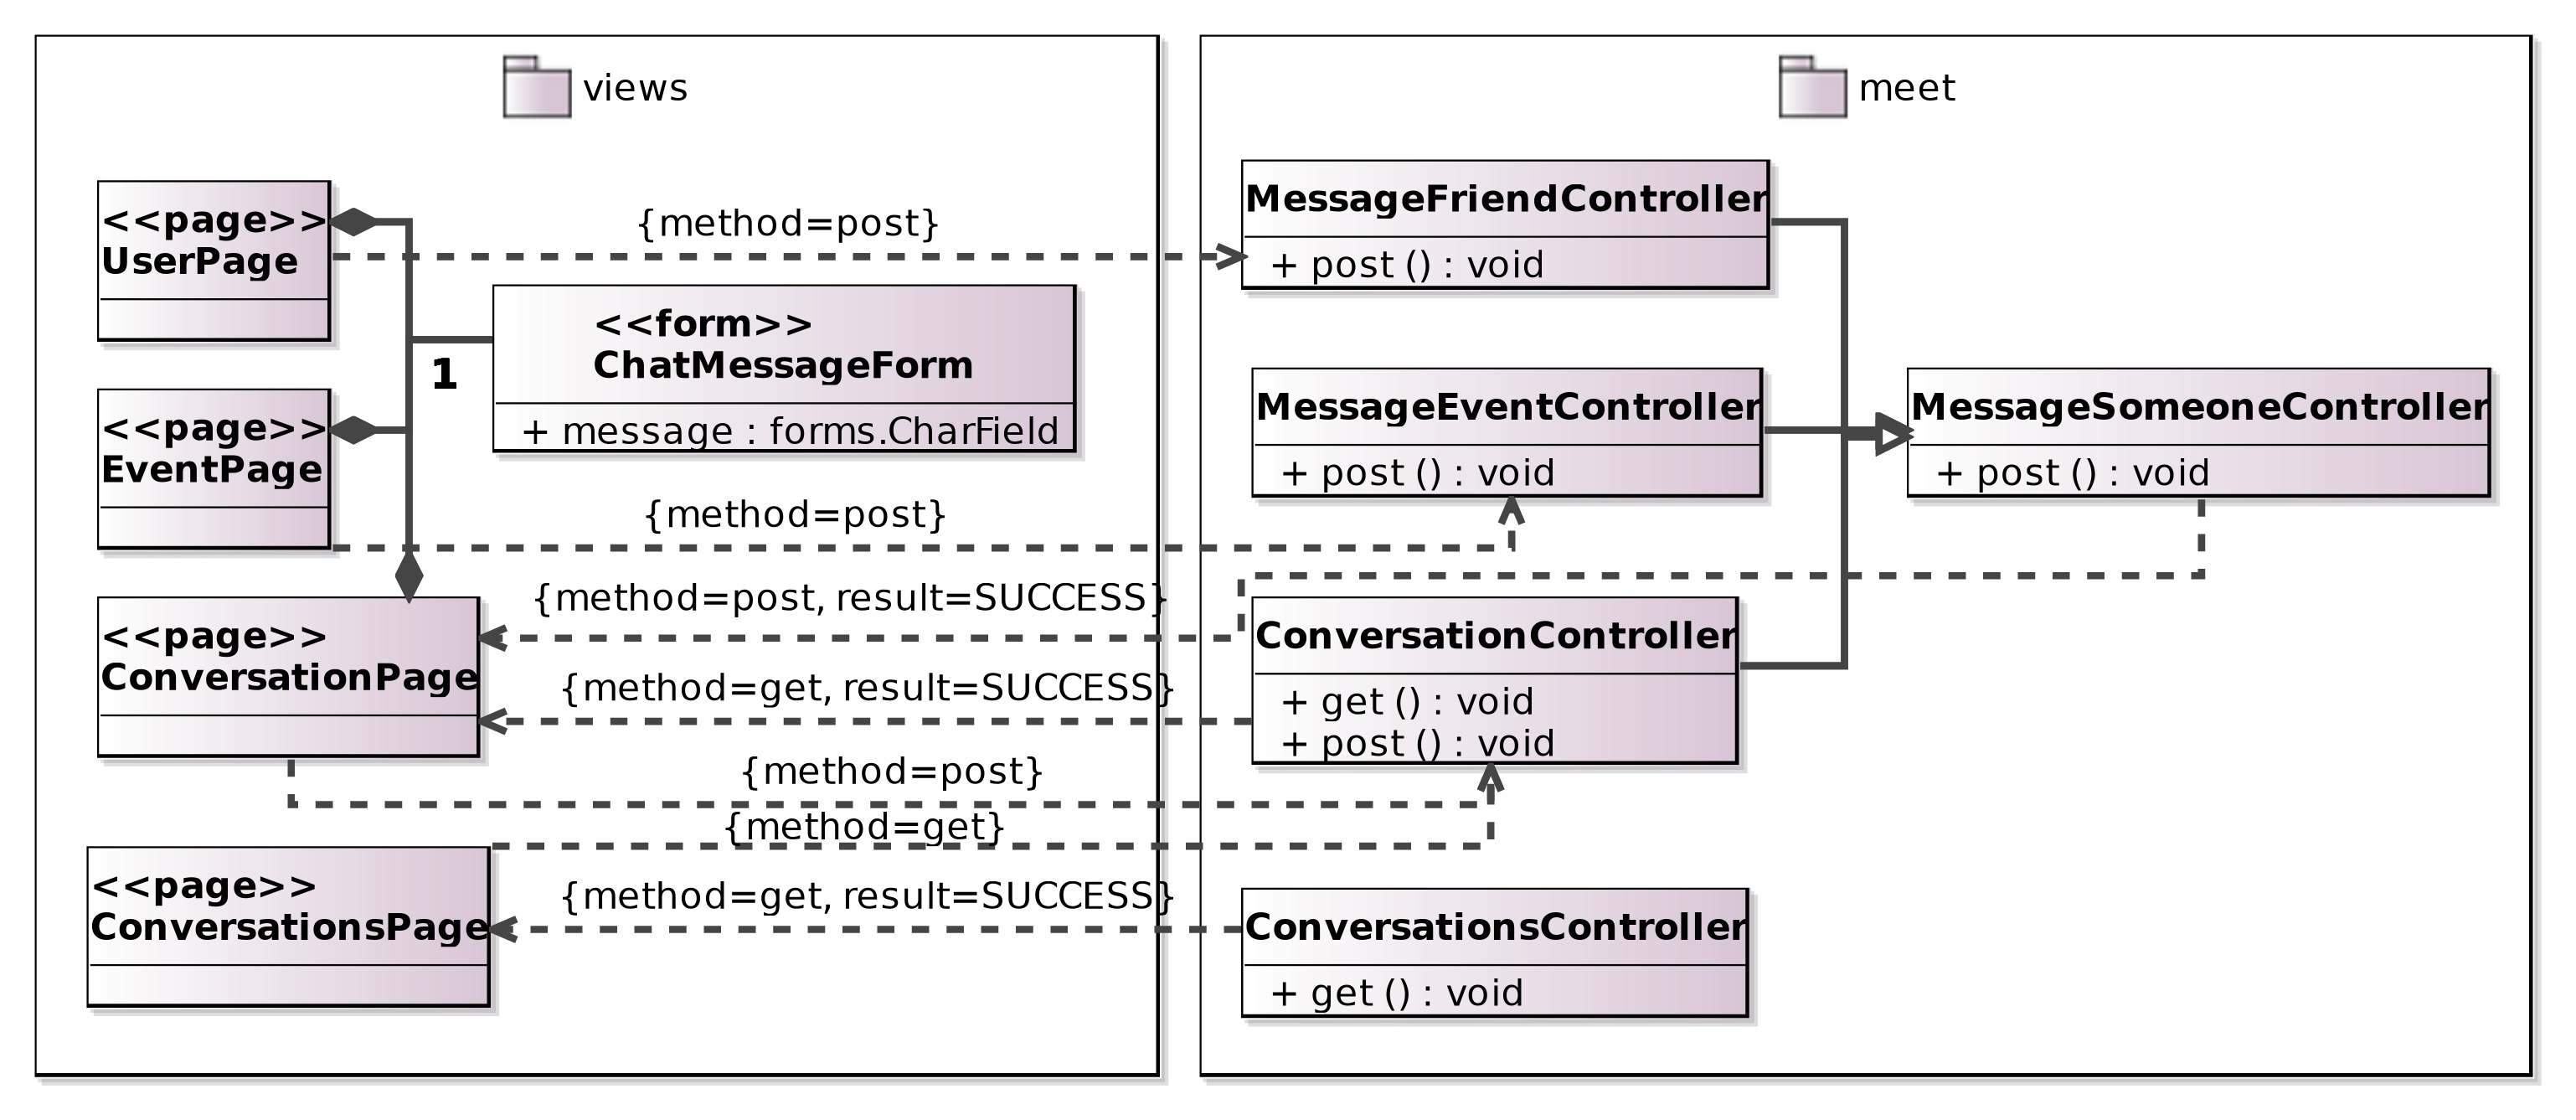
\includegraphics[scale=0.15]{figuras/FrameWebNavigationModel3.jpg}
	\caption{Modelo de Navegação do \imprimirtitulo{} -- Iniciar e continuar conversas}
	\label{fig:nav3}
\end{figure}

\begin{figure}[H]
	\centering
	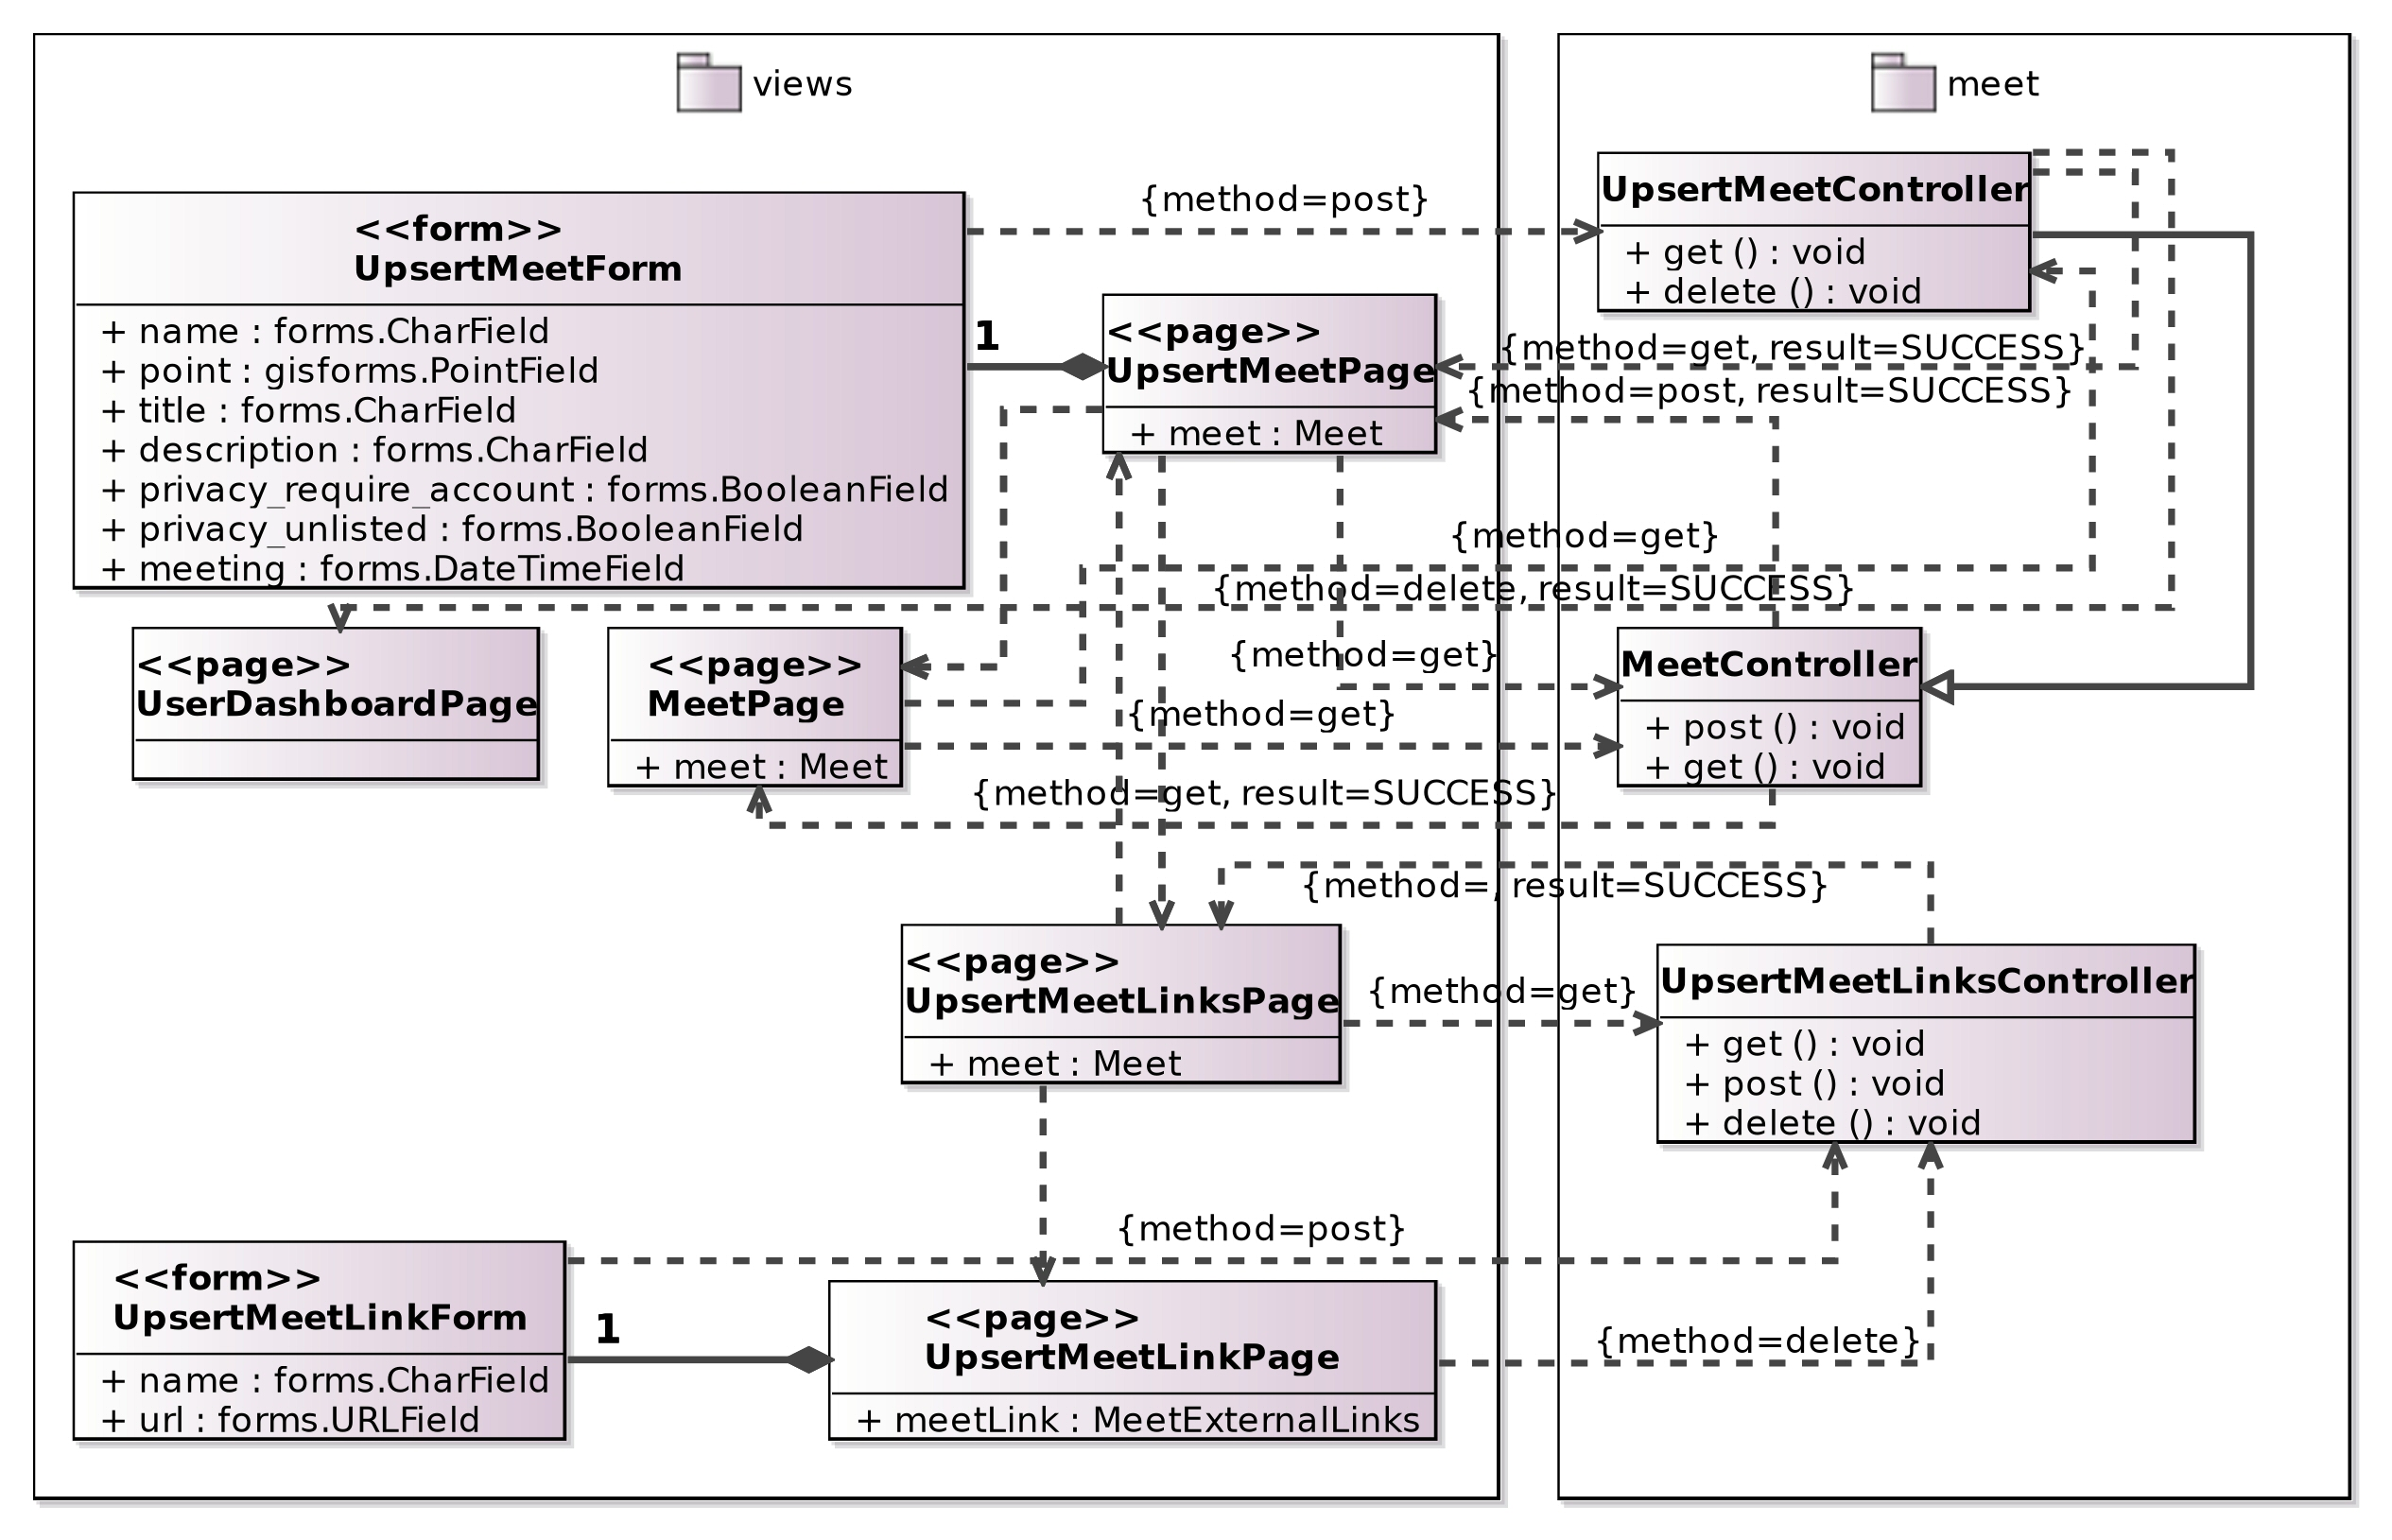
\includegraphics[scale=0.15]{figuras/FrameWebNavigationModel4.jpg}
	\caption{Modelo de Navegação do \imprimirtitulo{} -- Gerenciar encontros}
	\label{fig:nav4}
\end{figure}

\begin{figure}[H]
	\centering
	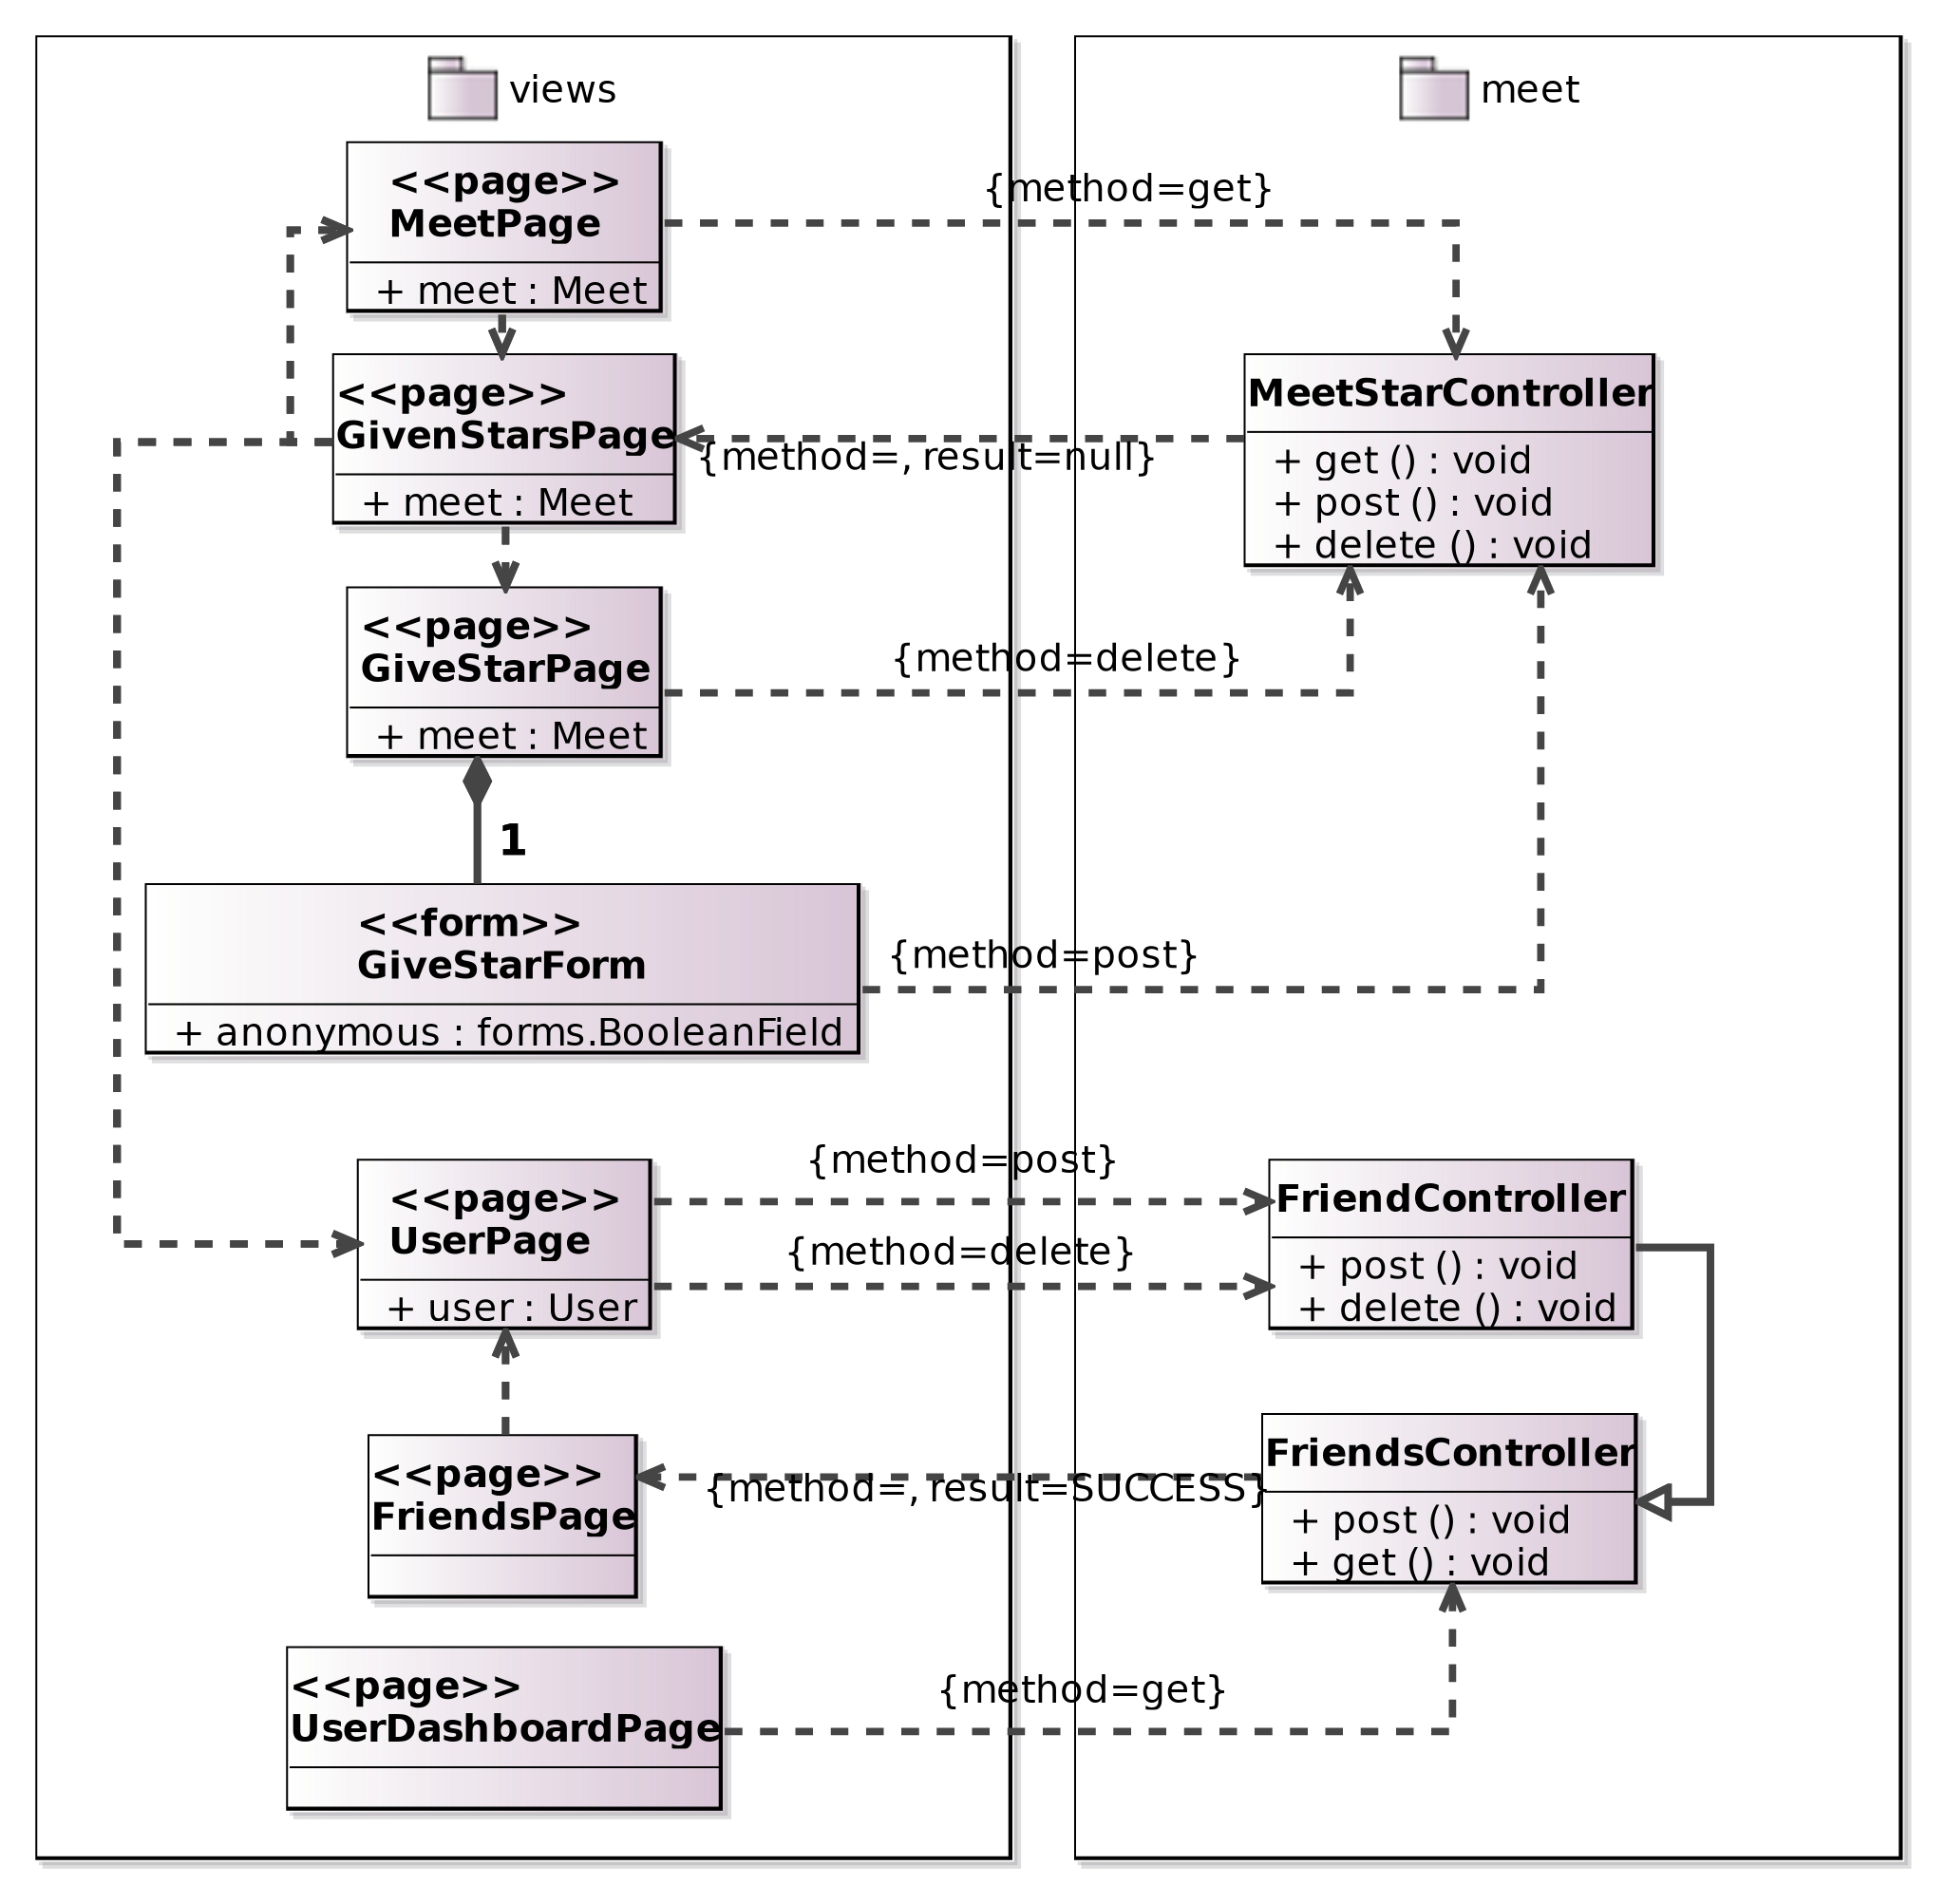
\includegraphics[scale=0.15]{figuras/FrameWebNavigationModel5.jpg}
	\caption{Modelo de Navegação do \imprimirtitulo{} -- Participar de encontros e adicionar/aceitar/rejeitar/desistir pedidos de amizade}
	\label{fig:nav5}
\end{figure}

\begin{figure}[H]
	\centering
	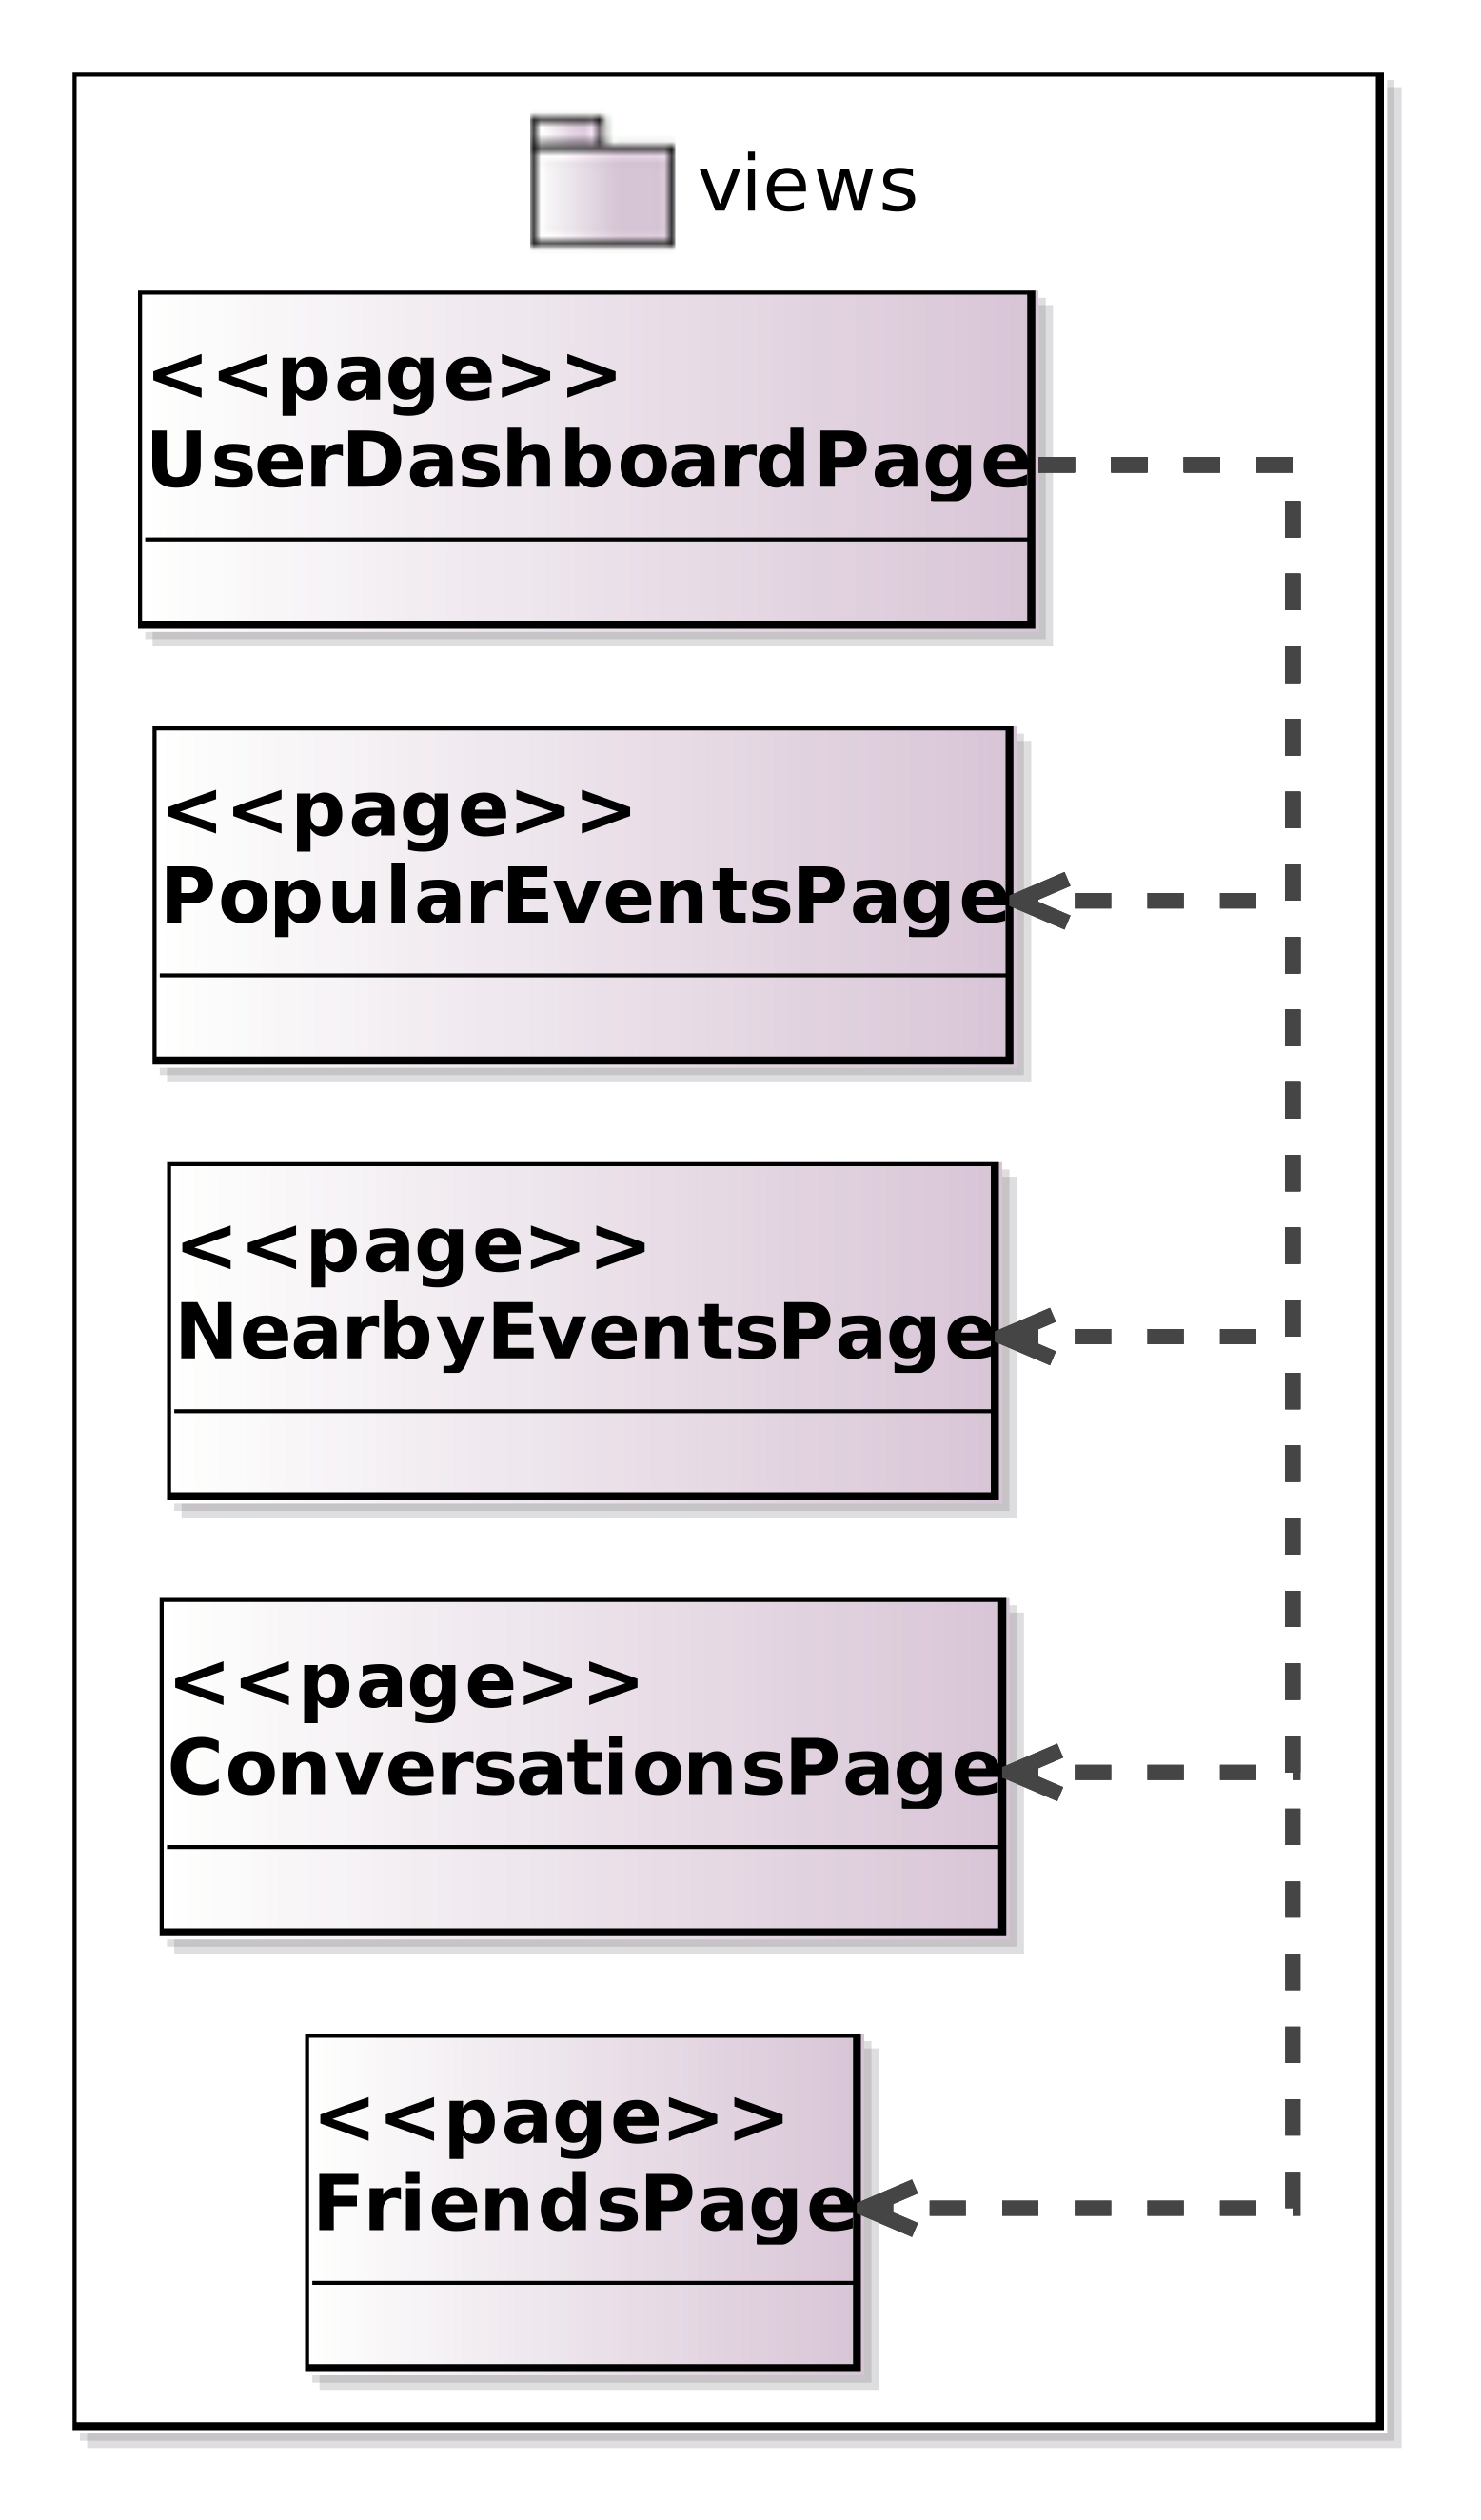
\includegraphics[scale=0.1]{figuras/FrameWebNavigationModel6.jpg}
	\caption{Modelo de Navegação do \imprimirtitulo{} -- O caminho do usuário de sua homepage até um ponto em comum com as funcionalidades mencionadas anteriormente; eventuais controladores foram omitidos}
	\label{fig:nav6}
\end{figure}




\section{Camada de Negócio}
\label{sec-arquitetura-negocio}

% \vitor{Apresentar os modelos de entidades e de aplicação do FrameWeb.}

\begin{figure}[H]
	\centering
	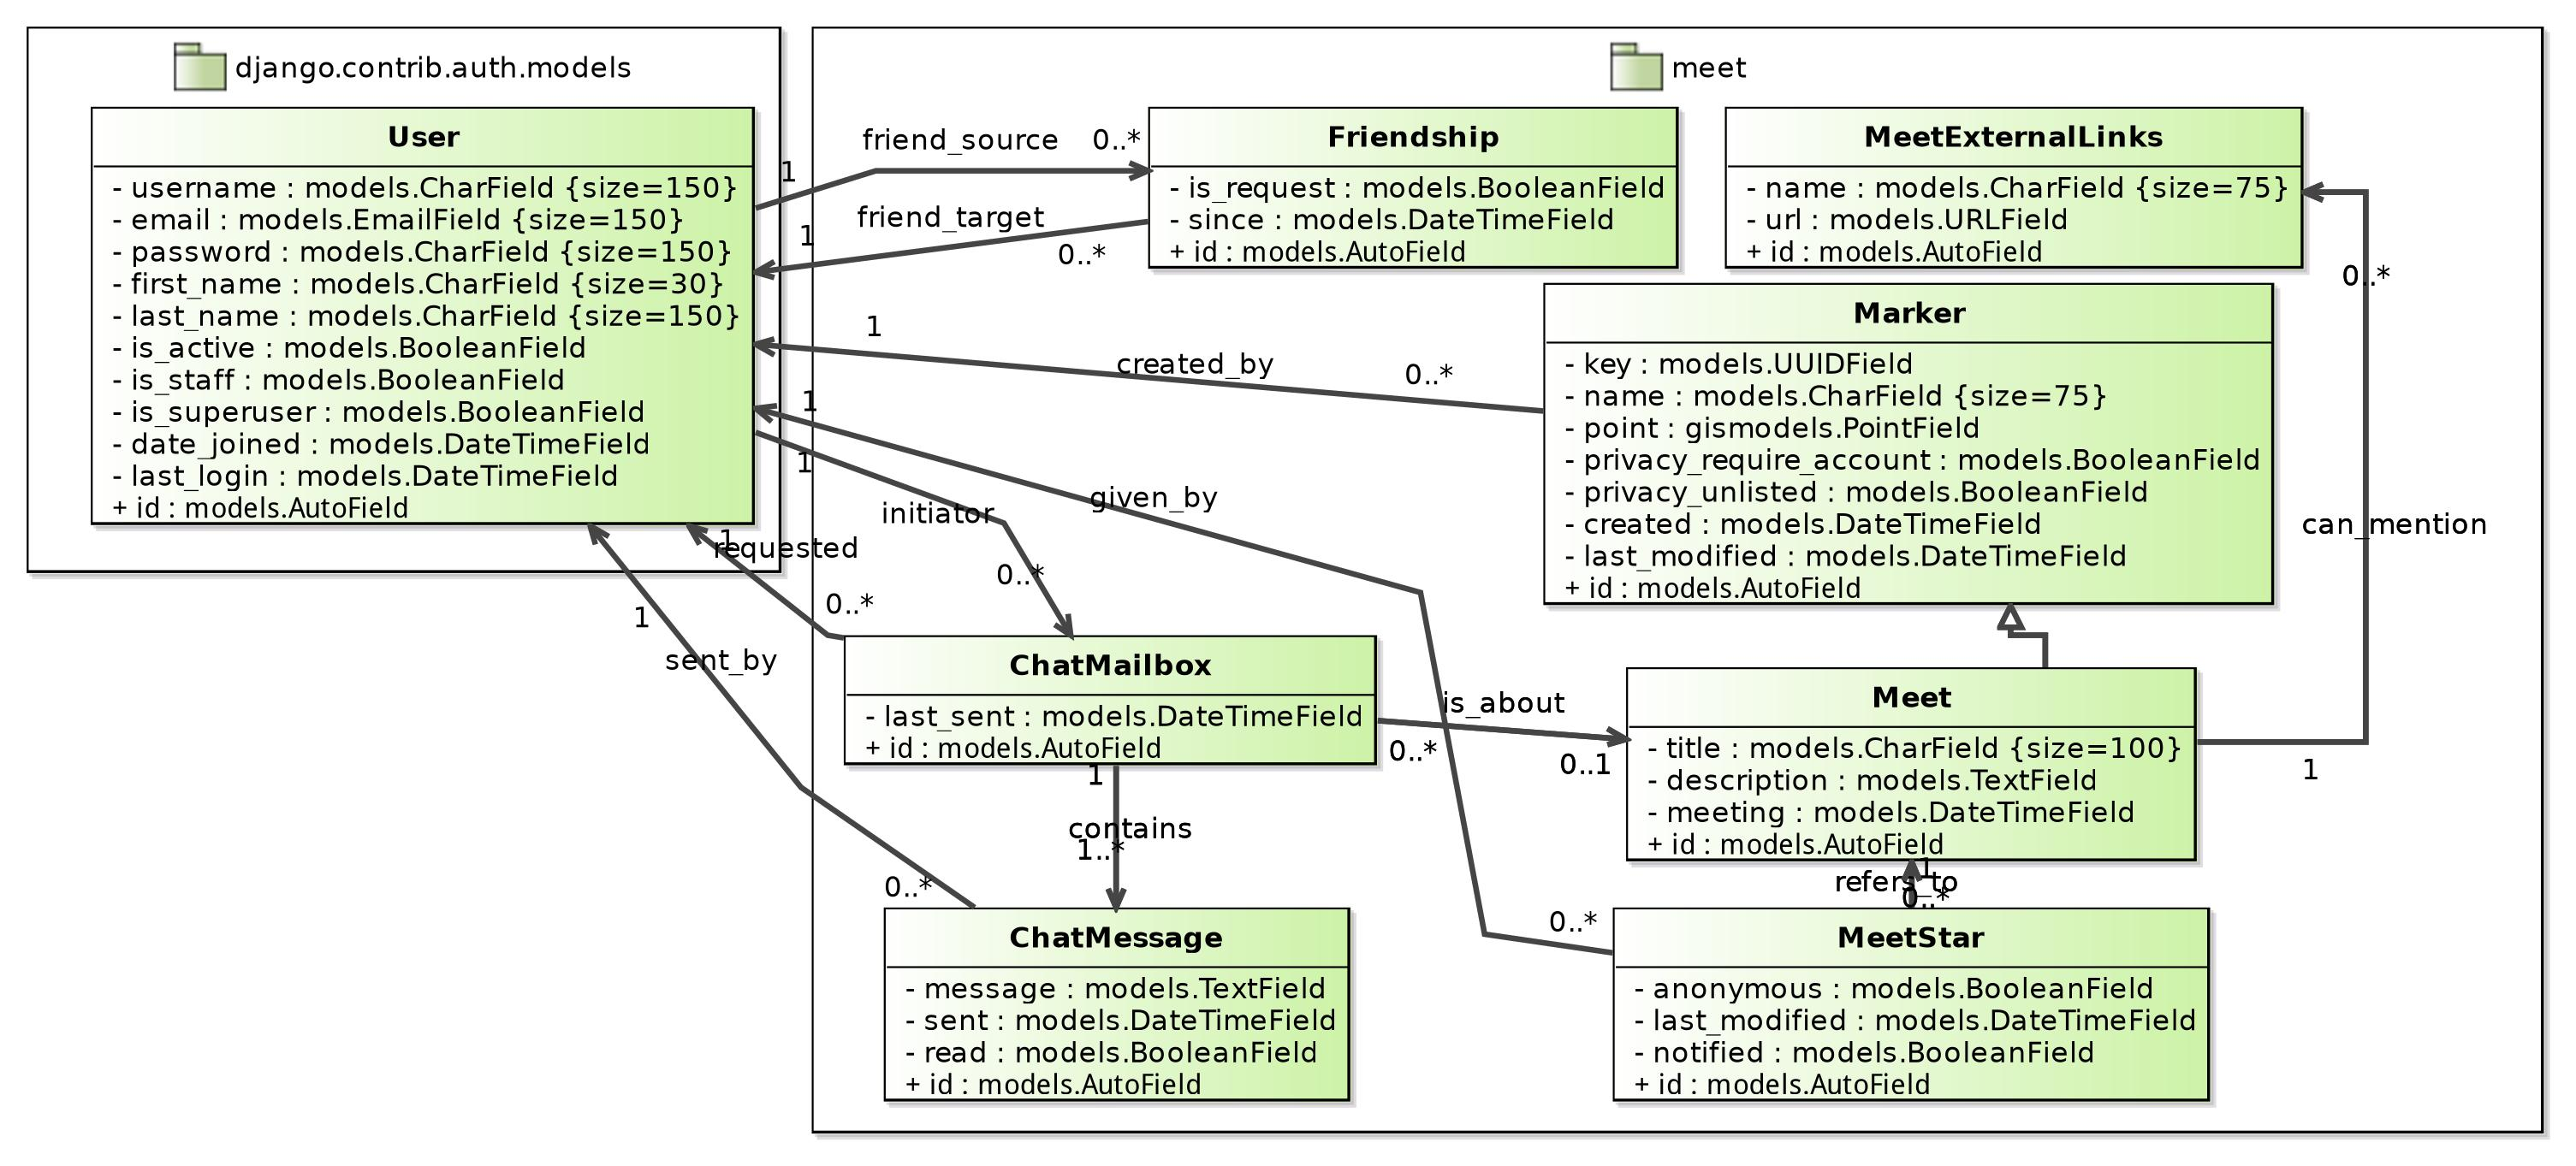
\includegraphics[width=0.8\textwidth]{figuras/FrameWebEntityModel.jpg}
	\caption{Modelo de Entidades do \imprimirtitulo.}
	\label{fig:ent}
\end{figure}

\begin{figure}[H]
	\centering
	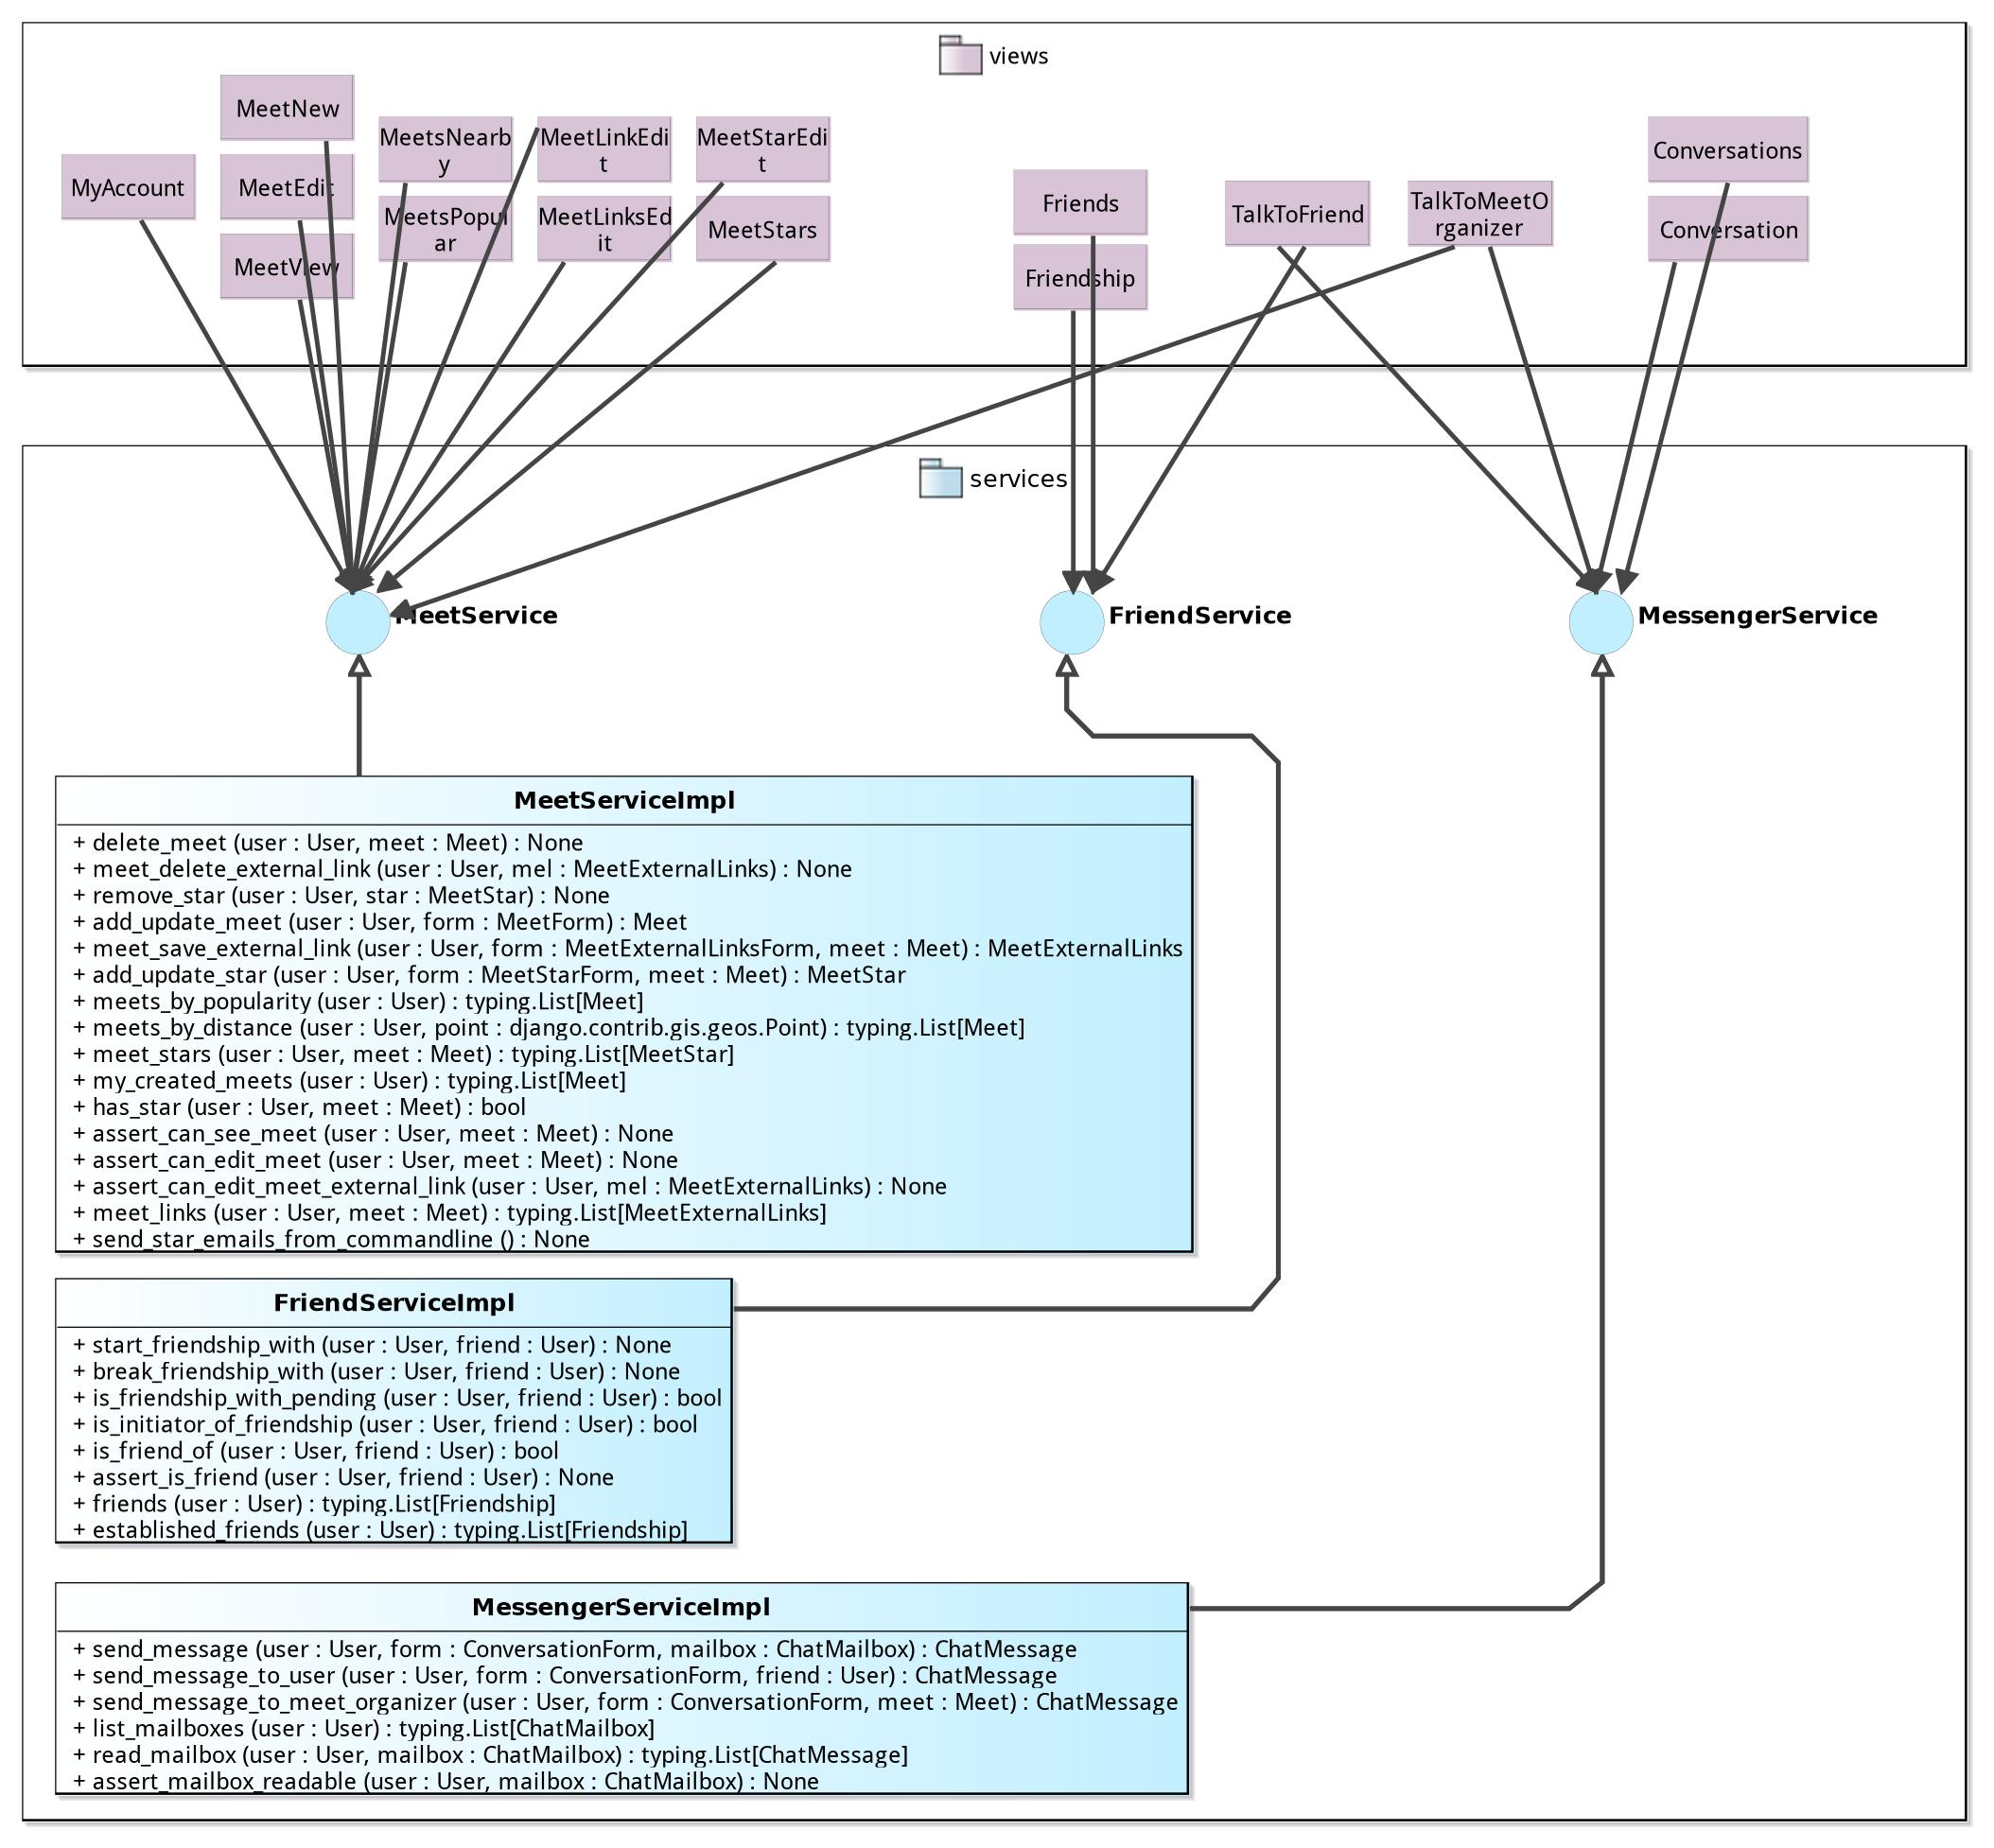
\includegraphics[width=0.8\textwidth]{figuras/FrameWebApplicationModel.jpg}
	\caption{Modelo de Aplicação do \imprimirtitulo.}
	\label{fig:apl}
\end{figure}




% \section{Camada de Acesso a Dados}
% \label{sec-arquitetura-dados}
%
% \vitor{Apresentar os modelos de persistência do FrameWeb.}
